\documentclass{book}

\PassOptionsToPackage{unicode,pdfusetitle}{hyperref}
\PassOptionsToPackage{hyphens}{url}
\PassOptionsToPackage{dvipsnames,svgnames,x11names}{xcolor}

% Small caps serif font, for Paper numbers, ISBN, etc
\newcommand{\I}{\textrm{\scshape i}\xspace}
\newcommand{\II}{\textrm{\scshape ii}\xspace}
\newcommand{\III}{\textrm{\scshape iii}\xspace}
\newcommand{\IV}{\textrm{\scshape iv}\xspace}
\newcommand{\V}{\textrm{\scshape v}\xspace}
\newcommand{\VI}{\textrm{\scshape vi}\xspace}
\newcommand{\VII}{\textrm{\scshape vii}\xspace}
\newcommand{\VIII}{\textrm{\scshape viii}\xspace}
\newcommand{\IX}{\textrm{\scshape ix}\xspace}
\newcommand{\X}{\textrm{\scshape x}\xspace}
\newcommand{\ISBN}{\textrm{\scshape isbn}\xspace}
\newcommand{\ISSN}{\textrm{\scshape issn}\xspace}

\usepackage{pageslts}

% G5 format
\usepackage[
  paperwidth=169mm,
  paperheight=239mm,
  nomarginpar,
]{geometry}

\usepackage[T1]{fontenc}
\usepackage{mathtools}
\usepackage[varqu,varl,scale=0.93]{inconsolata}
\usepackage[ebgaramond,textscale=0,semibold,vvarbb,amsthm]{newtx}
\usepackage[scale=0.9]{cabin}
\usepackage{bm}

\usepackage{pifont} % for dingbats

\usepackage{upquote} % straight quotes in verbatim environments
\usepackage{microtype}
\UseMicrotypeSet[protrusion]{basicmath} % disable protrusion for tt fonts

% Additional font sizes \HUGE and \ssmall, needed for figure captions
\usepackage{moresize}

% tikz and pgfplots
\usepackage{tikz}
\usetikzlibrary{calc,arrows,shapes,positioning,intersections}
\usepackage{pgfplots}
\usepgfplotslibrary{external,colormaps}
\pgfplotsset{compat=1.11}
\tikzexternalize[export=false]

\usepackage[labelfont=bf]{caption}
\usepackage[labelfont=bf]{subcaption}

\usepackage{epigraph}

% algorithms
\usepackage[ruled,vlined,linesnumbered]{algorithm2e}
% \usepackage{algpseudocode,algorithm}
% \resetcounteronoverlays{algocf}

\usepackage{xcolor}
\usepackage{xurl}
\usepackage{bookmark}
\usepackage{hyperref}

\definecolor{lublue}{RGB}{0,0,128}
\definecolor{lubronze}{RGB}{156,97,20}

\hypersetup{
  colorlinks = true,
  % hidelinks,
  breaklinks = true,
  linkcolor  = lublue,
  filecolor  = lublue,
  urlcolor   = lublue,
  citecolor  = lubronze
}
\usepackage{cleveref}

% Chapters should have numbers - a typical thesis consists of two chapters:
% One to introduce and summarize the research ("kappa"), and one for
% reproductions of the papers and manuscripts. No need to number them by default.
% If you need chapter numbers back, comment the following line.
\renewcommand{\thesection}{\arabic{section}}

% Sections and subsections have numbers, subsubsections etc do not.
% \setcounter{secnumdepth}{2}

% Only chapters and sections appear in the table of contents, not subsections etc
\addtocontents{toc}{\protect\setcounter{tocdepth}{1}}

% Ensures that \cleardoublepage inserts empty pages without page number
\usepackage{emptypage}

% For text macros (e.g., small caps macros)
\usepackage{xspace}

% For "Lorem Ipsum" style place holders
\usepackage{blindtext}

% For \includegraphics
\usepackage{graphicx}

% Nice looking tables with correct spacings 
\usepackage{booktabs}
\usepackage{multirow}

% Tables spanning more than one page
% \usepackage{longtable}

% Math symbols
% \usepackage{amsfonts,amsmath,amssymb}

% To include the PDFs of the papers
\usepackage[]{pdfpages}

% Hyphenation, support for different languages, last one is default
% Make sure to install the hyphenation packages for all languages you need
\usepackage[english]{babel}

% Figures can be kept in the same directory as the thesis, or in a Figure/
% directory, without need to specifying which of the two it is
\graphicspath{{figures/}}

%%%%%%%%%%%%%%%%%%%%%%%%%%%%%%%%%%%%%%%%%%%%%%%%%%%%%%%%%%%%%%%%%%%%
% define commands for chapters, sections, and subsections that do not
% have a number, but are entered as candidates for the table of contents.

\newcommand\chap[1]{%
  \chapter*{#1}%
  \addcontentsline{toc}{chapter}{#1}
  \markboth{#1}{#1}
}
\newcommand\sect[1]{%
  \section*{#1}%
  \addcontentsline{toc}{section}{#1}
  \markright{#1}
}
\newcommand\subsect[1]{%
  \subsection*{#1}%
  \addcontentsline{toc}{subsection}{#1}
}

% References should be a section of the summary text, with number and all ...
% \renewcommand\bibsection{\section{\bibname}\markright{\bibname}}

% code listings
\usepackage{listings}

% Define a custom color
\definecolor{backcolour}{rgb}{0.95,0.95,0.95}
\definecolor{codegreen}{rgb}{0,0.6,0}
\definecolor{mygray}{rgb}{0.6,0.6,0.6}

\lstdefinestyle{myStyle}{
  backgroundcolor=\color{backcolour},
  frame=single,
  % commentstyle=\color{codegreen},
  basicstyle=\ttfamily\small,
  breakatwhitespace=false,
  breaklines=true,
  keepspaces=true,
  numbers=left,
  % numbersep=5pt,
  numberstyle=\footnotesize\color{mygray},
  showspaces=false,
  showstringspaces=false,
  showtabs=false,
  tabsize=2,
}

% Use \lstset to make myStyle the global default
\lstset{style=myStyle}

\usepackage{enumitem}

\usepackage{siunitx}

\usepackage[
  style=authoryear-comp,
  language=english,
  url=false,
  sortcites=true,
  refsegment=chapter,
  % minbibnames=22,
  % mincitenames=22,
  % maxbibnames=22,
  % maxcitenames=25
]{biblatex}
\addbibresource{phdthesis.bib}

% Problem environment
\usepackage{aliascnt}
\newaliascnt{problem}{equation}
\aliascntresetthe{problem}
\creflabelformat{problem}{#2\textup{(#1)}#3}
\makeatletter
\def\problem{$$\refstepcounter{problem}}
\def\endproblem{\eqno \hbox{\@eqnnum}$$\@ignoretrue}
\makeatother
\Crefname{problem}{Problem}{Problems}

\usepackage{fancyhdr}
\renewcommand{\chaptermark}[1]{\markboth{#1}{}}
\renewcommand{\sectionmark}[1]{\markright{#1}}
\pagestyle{fancy}
\fancyhf{}
\fancyhead[LE,RO]{\thepage}
\fancyhead[LO]{\itshape\scshape\nouppercase{\rightmark}}
\fancyhead[RE]{\itshape\nouppercase{\leftmark}}
\renewcommand{\headrulewidth}{0pt}


% Re-usable information (title page, datasheet)
\newcommand{\myName}{Johan Larsson}
\newcommand{\myYear}{2024}
\newcommand{\myMainTitle}{Title}
\newcommand{\mySubTitle}{Subtitle}

% Compact combination of combining title and subtitle, used in datasheet and as
% chapter title for the main part.
\newcommand{\myTitle}{\myMainTitle: \mySubTitle}

\newcommand{\myFaculty}{Lund University School of Economics and Business Administration}
\newcommand{\myDepartment}{Department of Statistics}
\newcommand{\myAddress}{Box 7080\\SE--220 07 Lund\\Sweden} % Three lines maximum!

\newcommand{\myDegree}{Thesis for the degree of Doctor of Philosophy}
\newcommand{\myAdvisors}{Jonas Wallin and Małgorzata Bogdan}
\newcommand{\myOpponent}{TBA}

\newcommand{\myDefenceAnnouncement}{%
  To be presented, with the permission of the
  \myFaculty\xspace of Lund University, for public criticism in the Clark Kent
  lecture hall (Kentsalen) at the \myDepartment\xspace
  on Sunday, the 34th of December \myYear\xspace at 24:00. }
\newcommand{\myCoverFront}{%
  \noindent {\bf Cover illustration front:}
  A really pretty thing that looks great on the front but has only a
  remote connection to do with my research (Credits: The awesome person who made
  this picture).}
\newcommand{\myCoverBack}{%
  {\bf Cover illustration back:} Picture showing my research (Paper \V).}
\newcommand{\myFundingInformation}{%
  {\bf Funding information:}
  The thesis work was financially supported by my rich uncle.}

\newcommand{\mySeries}{%
  \ISSN: $<$ISSN number$>$}

\newcommand{\myISBNprint}{1234567890}
\newcommand{\myISBNpdf}{0987654321}
\newcommand{\myFormSignDate}{1776-7-4}

% total page number is computed automatically:
\newcommand{\myPages}{\lastpageref{LastPages}}

\newcommand{\myFormDefenceDate}{2015-12-24}
\newcommand{\myFormKeywords}{%
  power, victory, awesomeness}

% Write a short english abstract of the thesis here, goes into the data sheet page 4. 
\newcommand{\myAbstract}{
  \blindtext

  \blindtext
}%

% --- Shortcut thesis commands for paper references and titles ---
% Included papers - only need to type this once
\newcommand{\PaperIauthor}{\textbf{F. Lastname}, C. Coauthor, \ldots}
\newcommand{\PaperIIauthor}{\textbf{F. Lastname}, C. Coauthor, \ldots}
\newcommand{\PaperIIIauthor}{\textbf{F. Lastname}, C. Coauthor, \ldots}
\newcommand{\PaperIVauthor}{\textbf{F. Lastname}, C. Coauthor, \ldots}
\newcommand{\PaperVauthor}{\textbf{F. Lastname}, C. Coauthor, \ldots}
\newcommand{\PaperVIauthor}{\textbf{F. Lastname}, C. Coauthor, \ldots}

\newcommand{\PaperIref}{Journal for Superheroes, pp. 1--10}
\newcommand{\PaperIIref}{Journal for Bankers, pp. 2--30}
\newcommand{\PaperIIIref}{Journal for Superheroes, pp. 1--10}
\newcommand{\PaperIVref}{Journal for Superheroes, pp. 1--10}
\newcommand{\PaperVref}{Journal for Superheroes, pp. 1--10}
\newcommand{\PaperVIref}{Journal for Superheroes, pp. 1--10}

\newcommand{\PaperItitle}{Spiderman vs Superman}
\newcommand{\PaperIItitle}{On the matter of \ldots}
\newcommand{\PaperIIItitle}{On the matter of \ldots}
\newcommand{\PaperIVtitle}{On the matter of \ldots}
\newcommand{\PaperVtitle}{On the matter of \ldots}
\newcommand{\PaperVItitle}{On the matter of \ldots}

% Not included papers, in case you want to list them
%\newcommand{\PaperNotIncIauthor}{C. Coauthor, \textbf{X. Someone}}
%\newcommand{\PaperNotIncIref}{Journal for \ldots}
%\newcommand{\PaperNotIncItitle}{Boring matter}
% --- END reusable thesis commands ---

\begin{document}

%%%%%%%%%%%%% First pages with thesis title etc %%%%%%%%%%%%%%%%%%%%%%%%%%%%%%%%
% First six pages are contained in a separate file. Normally you should not
% need to edit it.

\pagestyle{empty}

% This file contains the layout of the first six pages and the explanation text
% of a compilation thesis. 

%%%%%%%%%%%%% FIRST PAGES WITH THESIS TITLE ETC %%%%%%%%%%%%%%%%%%%%%%%%%%%%%%%%
\frontmatter % roman numbers

% Page one: Title only
\thispagestyle{empty} % no page number
\begin{center}
  \vspace*{5cm}
  {\Large \myMainTitle}
  %\\
  %{\large \mySubTitle}
\end{center}

% Page two: empty. Empty space is important

%%%%%%%%%%%%%%%%%%%%%%%%%%%%%%%%%%%%%%%%%%%%%%%%%%%%%%%%%%%%%%%%%%%%%%%
% Page three: title page with small text (spikningsblad)

\cleardoublepage
\thispagestyle{empty} % no page number
~
\vfill
\begin{center}
  {\HUGE \myMainTitle}
  \\[2mm]
  {\huge \mySubTitle}

  \vfill
  {\myName}

  \vfill
  % black and white (default):
  
\includegraphics[width=0.25\textwidth]{LundUniversity_C2line_BLACK.eps}

  \vspace{10mm}
  {\large \myDegree}\\
  {\large Thesis advisors: \myAdvisors}\\
  {\large Faculty opponent: \myOpponent}\\
  \vspace{1cm}
  {\footnotesize
    \myDefenceAnnouncement
  }
  \\
\end{center}
\vfill

%%%%%%%%%%%%%%%%%%%%%%%%%%%%%%%%%%%%%%%%%%%%%%%%%%%%%%%%%%%%%%%%%%%%%%%
% Page four: data sheet
\newpage

%Either include datasheet texfile (will be filled in automatically), or a pdf
%containing datasheet (text needs to be already in it, edit
%sheetPDF_editable.pdf). Use one of the next two lines: 
\newcounter{aformdx}
\newcounter{aformdy}
\newcounter{aformx}
\newcounter{aformy}
\newcounter{aformtx}
\newcounter{aformtdx}
\newcounter{aformty}
\def\aformw{358}
\def\aformwhalf{\aformw / 2}
\def\aformwquart{\aformw / 4}
\def\aformwthreeq{\aformw / 4 * 3}
\def\aformh{517}
\def\aformb{23}
\def\aformlinew{0.4pt}
\def\aformrowh{20}
\def\aformRowh{24}
\newcommand\aformhline
{\put(\value{aformx},\value{aformy}){\line(1,0){\value{aformdx}}}}
\newcommand\aformvline
{\put(\value{aformx},\value{aformy}){\line(0,-1){\value{aformdy}}}}
\newcommand\aformvlinec
{\put(\value{aformx},\value{aformy}){\line(0,-1){16.25}}}
\newcommand\aformboxbase[5]
{
  \setcounter{aformtx}{\value{aformx}}
  \setcounter{aformtdx}{\value{aformdx}}
  \setcounter{aformty}{\value{aformy}}
  \addtocounter{aformtx}{#1}
  \addtocounter{aformtdx}{-#2}
  \addtocounter{aformty}{-#3}
  \put(\value{aformtx},\value{aformty})
  {
    \parbox[t]{\value{aformtdx}pt}
    {{\sf\tiny #4}{\scriptsize #5\par}}
  }
}
\newcommand\aformbox[2]{\aformboxbase{2}{11}{8}{#1}{#2}}
\newcommand\aformBox[2]{\aformboxbase{2}{11}{8}{#1}{#2}}

\begin{center}
  \begin{picture}(\aformw,510)(0,0)
    \linethickness{\aformlinew}
    \put(0,\aformb){\framebox(\aformw,\aformh){}}
    \put(-14,200){\rotatebox{90}{\parbox{200pt}
        {\sf\tiny
          DOKUMENTDATABLAD
          enl SIS 61 41 21\\
        }}}
    \setcounter{aformx}{0}
    \setcounter{aformy}{\aformb}
    \addtocounter{aformy}{\aformh}
    \setcounter{aformdx}{\aformwhalf}
    \aformbox{Organization}
    {\\
    {\bf LUND UNIVERSITY}\vspace{0.1cm}
    \\
    {\myDepartment\\
    \myAddress}
    }
    \setcounter{aformdy}{\aformrowh}
    \addtocounter{aformdy}{\aformrowh}
    \addtocounter{aformdy}{\aformrowh}
    \addtocounter{aformdy}{\aformRowh}
    \setcounter{aformx}{\aformwhalf}
    \aformvline
    \setcounter{aformx}{0}
    \addtocounter{aformy}{-\aformrowh}
    \addtocounter{aformy}{-\aformrowh}
    \addtocounter{aformy}{-\aformRowh}
    \aformbox{Author(s)}{\\\myName}
    \setcounter{aformdy}{\aformrowh}
    \aformhline
    \addtocounter{aformy}{\aformrowh}
    \addtocounter{aformy}{\aformrowh}
    \addtocounter{aformy}{\aformRowh}
    \setcounter{aformx}{\aformwhalf}
    \aformbox{Document name}{\\{\bf DOCTORAL DISSERTATION}}
    \addtocounter{aformy}{-\aformrowh}
    \aformhline
    \aformbox{Date of disputation}{\\\myFormDefenceDate}
    \setcounter{aformx}{\aformwhalf}
    \aformhline
    \addtocounter{aformy}{-\aformrowh}
    \addtocounter{aformdy}{\aformRowh}
    \aformbox{Sponsoring organization}{}
    \aformhline
    \addtocounter{aformy}{-\aformRowh}
    \addtocounter{aformy}{-\aformrowh}
    \setcounter{aformx}{0}
    \setcounter{aformdx}{\aformw}
    \aformhline
    \aformbox{Title and subtitle }{\\\myTitle}
    \addtocounter{aformy}{-\aformRowh}
    \setcounter{aformx}{0}
    \aformhline
    \aformBox{Abstract}
    {\\
    {\parskip0pt\parindent1em
    \myAbstract
    }
    }
    \setcounter{aformy}{\aformb}
    % Correspond to one minus each in the bottom section
    \addtocounter{aformy}{\aformRowh}
    \addtocounter{aformy}{\aformRowh}
    \addtocounter{aformy}{\aformRowh}
    \addtocounter{aformy}{\aformRowh}
    \addtocounter{aformy}{\aformrowh}
    \addtocounter{aformy}{\aformrowh}
    \addtocounter{aformy}{10}
    \addtocounter{aformy}{10}
    \aformhline
    \aformbox{Key words}
    {
      \\\myFormKeywords
    }
    \addtocounter{aformy}{-\aformRowh}
    \addtocounter{aformy}{-10}
    \aformhline
    \aformbox{Classification system and/or index terms (if any)}{}
    \addtocounter{aformy}{-\aformRowh}
    \aformhline
    \aformbox{Supplementary bibliographical information}{}
    \setcounter{aformx}{\aformwthreeq}
    \setcounter{aformdx}{\aformwquart}
    \setcounter{aformdy}{\aformRowh}
    \aformvline
    \aformbox{Language}{\\English}
    \addtocounter{aformy}{-\aformRowh}
    \setcounter{aformx}{0}
    \setcounter{aformdx}{\aformw}
    \aformhline
    \aformbox{ISSN and key title}{}
    \setcounter{aformx}{\aformwthreeq}
    \addtocounter{aformdy}{10}
    \aformvline
    \addtocounter{aformdy}{-10}
    \aformbox{ISBN}{\\\myISBNprint\xspace(print)\\\myISBNpdf\xspace(pdf)}
    \addtocounter{aformy}{-\aformRowh}
    \addtocounter{aformy}{-10}
    \setcounter{aformx}{0}
    \aformhline
    \aformbox{Recipient's notes}{}
    \setcounter{aformx}{\aformwhalf}
    \setcounter{aformdy}{\aformrowh}
    \addtocounter{aformdy}{\aformrowh}
    \aformvline
    \aformbox{Number of pages}{\\227}
    \setcounter{aformx}{\aformwthreeq}
    \aformbox{Price}{}
    \setcounter{aformdy}{\aformrowh}
    \aformvline
    \addtocounter{aformy}{-\aformrowh}
    \setcounter{aformx}{\aformwhalf}
    \setcounter{aformdx}{\aformwhalf}
    \aformhline
    \aformbox{Security classification}{}
    \setcounter{aformx}{0}
    \setcounter{aformdx}{\aformw}
    \addtocounter{aformy}{-\aformrowh}
    \addtocounter{aformy}{-4}
    \aformbox{}
    {\scriptsize I, the undersigned, being the copyright owner of the abstract of the
      above-mentioned dissertation, hereby grant to all reference sources
      the permission to publish and disseminate the abstract of the
      above-mentioned dissertation.
    }
    \addtocounter{aformy}{-\aformRowh}
    \addtocounter{aformy}{-20}
    \aformbox{
      \hspace{0pt}
      %\put(44,1){\includegraphics{images/signature}} %Media-Tryck does not want this to be included as a graphic
    }{}
    \aformbox{\rm
      \scriptsize
      Signature \underline{\hskip 140pt}\hfill Date \underline{\hskip 80pt}
    }{}
    \addtocounter{aformy}{1}
    \aformbox{}{\hskip 280pt \scriptsize \myFormSignDate}
  \end{picture}
\end{center}

%\addtocounter{pages}{1} 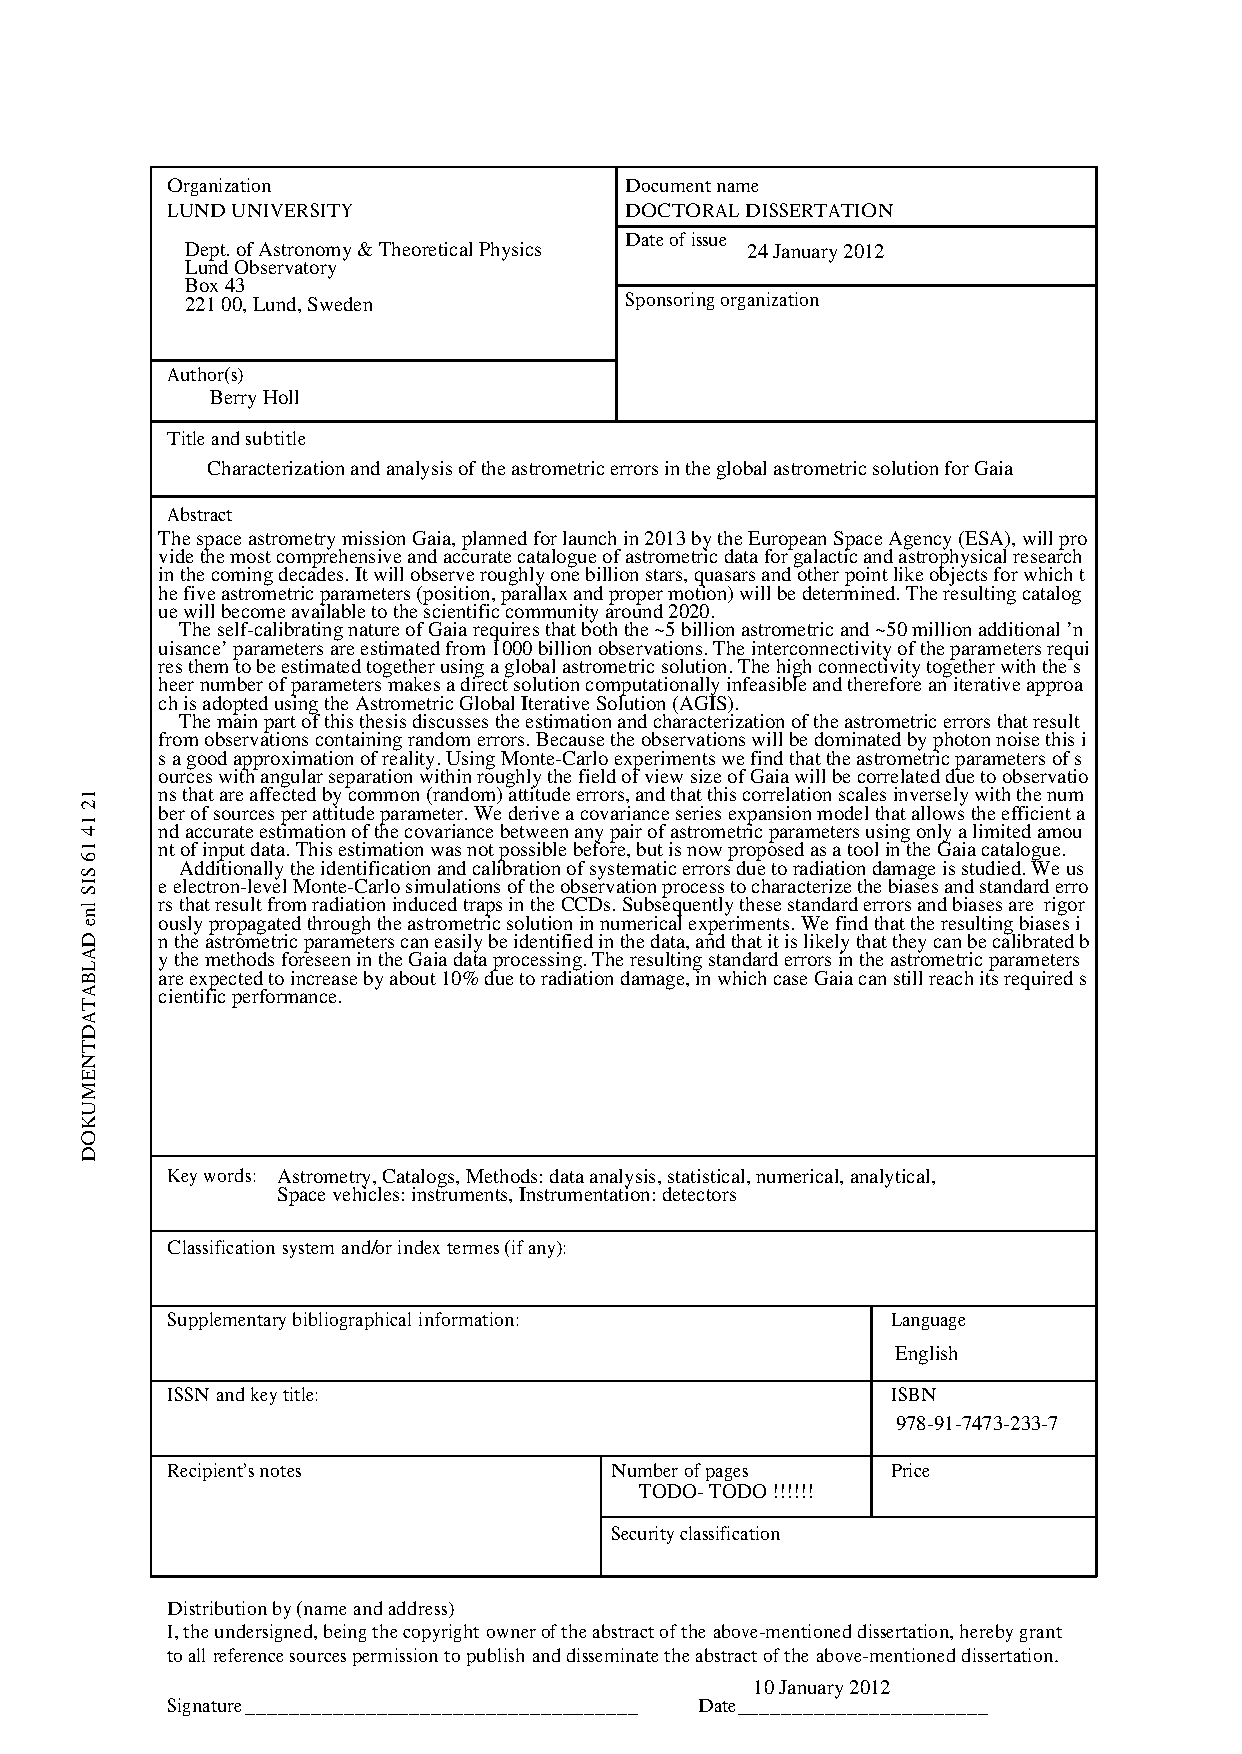
\includepdf[pages=1-1]{datasheetPDF_editable}

%%%%%%%%%%%%%%%%%%%%%%%%%%%%%%%%%%%%%%%%%%%%%%%%%%%%%%%%%%%%%%%%%%%%%%%
% Page five: title and author, without small text. Looks good!

\cleardoublepage
\thispagestyle{empty} % no page number
~
\vfill
\begin{center}
  {\HUGE \myMainTitle}
  \\[2mm]
  {\huge \mySubTitle}

  \vfill
  {\myName}

  \vfill
  % black and white (default):
  
\includegraphics[width=0.25\textwidth]{LundUniversity_C2line_BLACK.eps}

  % Colour text in white so that the spacing is the same as on page three, but with less clutter
  \color{white}{
  \vspace{10mm}
  {\large \myDegree}\\
  {\large Thesis advisors: \myAdvisors}\\
  {\large Faculty opponent: \myOpponent}\\
  \vspace{1cm}
  {\footnotesize
    \myDefenceAnnouncement
  }
  }
  \\
\end{center}
\vfill


%%%%%%%%%%%%%%%%%%%%%%%%%%%%%%%%%%%%%%%%%%%%%%%%%%%%%%%%%%%%%%%%%%%%%%%
% Page six: Cover image description, ISBN, copyright
\newpage

\thispagestyle{empty} % no page number

\noindent A doctoral thesis at a university in Sweden takes either the form of a single,
cohesive research study (monograph) or a summary of research papers
(compilation thesis), which the doctoral student has written alone or together
with one or several other author(s).

In the latter case the thesis consists of two parts. An introductory text puts
the research work into context and summarizes the main points of the papers.
Then, the research publications themselves are reproduced, together
with a description of the individual contributions of the authors. The
research papers may either have been already published or are manuscripts at
various stages (in press, submitted, or in draft).

\vfill
{\small
  \myCoverFront\\
  \\
  \myCoverBack\\
  \\
  \myFundingInformation


  \vspace{5mm}
  \noindent\copyright\, \myName~\myYear\\
  \\
  \myFaculty, {\myDepartment}
  \\
  \\
  \ISBN: \myISBNprint~(print)\\ % ISBN av svenska ISBN centralen
  \ISBN: \myISBNpdf~(pdf)\\ % ISBN av svenska ISBN centralen
  \mySeries\\
  \\
  Printed in Sweden by Media-Tryck, Lund~University, Lund~\myYear

  \medskip

  \noindent
\includegraphics[width=0.5\textwidth]{ENG-Miljologotyper-sid-2-BLACK.eps}
}


% ===============================================================
% ===================== INSPIRATIONAL QUOTE:  ===================
% ===============================================================
\newpage
\thispagestyle{empty} % No page number on quote page
~
\vspace{140pt}
\begin{flushright}
  \textit{Dedicated to my siblings\\Name -- Name -- Name}
\end{flushright}

\cleardoublepage

\pagestyle{headings}

% Table of Contents
\setcounter{page}{1} % Page Roman 1 of the frontmatter
\setcounter{tocdepth}{1}

\tableofcontents
\addtocontents{toc}{\protect\thispagestyle{empty}}

%%%%%%%%%%%%%%%%%%%%%%%%%%%%%%%%%%%%%%%%%%%%%%%%%%%%%%%%%%%%%%%%%%%%
%%%%%%%%%%% List of publications %%%%%%%%%%%%%%%%%%%%%%%%%%%
% Have a long list and want to start on the left page? Here, have a special
% chapter heading for that!
%\addcontentsline{toc}{part}{Part 1: Summary}
%\renewcommand{\chapterheadstartvskip}{}
%{\let\cleardoublepage\relax \let\chapterheadstartvskip\nop 

\newpage

\chap{Acknowledgements}

This template was created and shared as a private initiative and comes without
support of any kind. If you are happy to have it, you are welcome to say thanks
and/or to send beers/goodies! :)

\newpage

\chap{Abstract}

Need more languages? Go to preamble.tex and add them to the
usepackage[\ldots]{babel} line. Install the corresponding packages on your
system.

\chap{List of Publications\label{sec:paperlist}}

This thesis is based on the following publications.

\begin{description}[leftmargin=!,labelwidth=0.7cm]
  \item[\I]  \fullcite{larsson2020b}
  \item[\II] \fullcite{larsson2021}
  \item[\III] \fullcite{larsson2022b}
  \item[\IV] \fullcite{moreau2022a}
  \item[\V] \fullcite{larsson2023}
\end{description}

%   % Publications not included in this thesis:
%   % \vspace{2mm}
%   %
%   % \begin{tabularx}{\textwidth}{rX}
%   % {\sc \phantom{vi}}   & {\bf \PaperNotIncItitle}\\[2mm]
%   %	  & \PaperNotIncIauthor\\
%   %          & \PaperNotIncIref\\[5mm] 
%   %
%   %\end{tabularx}
%   %
% } % End large font tables, continue with font size stated in preamble

\noindent {\small All papers are reproduced with permission of their respective publishers.}

% Page numbers arabic 
\mainmatter
% Reset table counters to not count the publications table
\setcounter{table}{0}
% Rest page counters, this is where it all starts!
\setcounter{page}{1}

\chap{\myTitle}
% Fancy a quote?
%\begin{flushright}
%\textit{It's easy to be complicated\\but very difficult to be simple.}\\
%{--- Debasish Mridha}
%\\[1cm]
%\textit{Everything should be made as simple as possible, but not simpler}\\
%{--- Albert Einstein}
%\end{flushright}
\section{Introduction}
\subsection{Foo bar}

\blindtext[3]

\subsection{Baz Baf\label{sec:mainresults}}
\begin{figure}
  
\includegraphics[width=0.6\textwidth]{natfak}
  \caption{The Faculty of Science and the Astronomy tower. (Figure: Lund University)\label{fig:cool}}
\end{figure}

Explaining something cool (\Cref{fig:cool}), which can be seen in a fantastic reference
\parencite{bogdan2015}. Figures and tables are placed automatically, such that they are
close by but not necessarily on the same page\footnote{to optimize page space}.


The concepts are summarized in Table~\ref{tab:comparison}.

\begin{table}[htb]
  \caption{Table caption with a CAPS word, no small caps can be used in table and figure captions because sans serif fonts don't support it.\label{tab:comparison}}
  \centering
  \begin{tabular}{lcccc}
    \toprule
              & Superman    & Spiderman     \\
    \midrule
    Gender    & male        & male          \\
    Species   & Homo Sapien & Human/spider  \\
    Homeworld & Gotham City & Earth         \\
    \midrule
    Publisher & DC Comics   & Marvel Comics \\
    \bottomrule
  \end{tabular}
\end{table}

\section{Some more background}

\blindtext[10]

\section{Main results of the research papers}

\blindtext

\printbibliography

\chap{Papers}

\cleardoublepage
\addcontentsline{toc}{section}{Paper~\I: {\PaperItitle}}

\thispagestyle{empty}

\begin{tikzpicture}[remember picture, overlay]
  \node[fill=black, text=white, font=\bfseries\fontsize{50}{55}\selectfont, anchor=east, minimum height=1.5cm, minimum width=2.5cm, text width=1.5cm, align=left] at ($(current page.north east) + (0,-0.2\paperheight)$) {\I};
\end{tikzpicture}

\cleardoublepage
% Include the PDF. Comment this while writing the thesis, only add later. 
% Options are: all pages, scaled to full width (use 0.95 if that is too high for some reason), with thesis page number
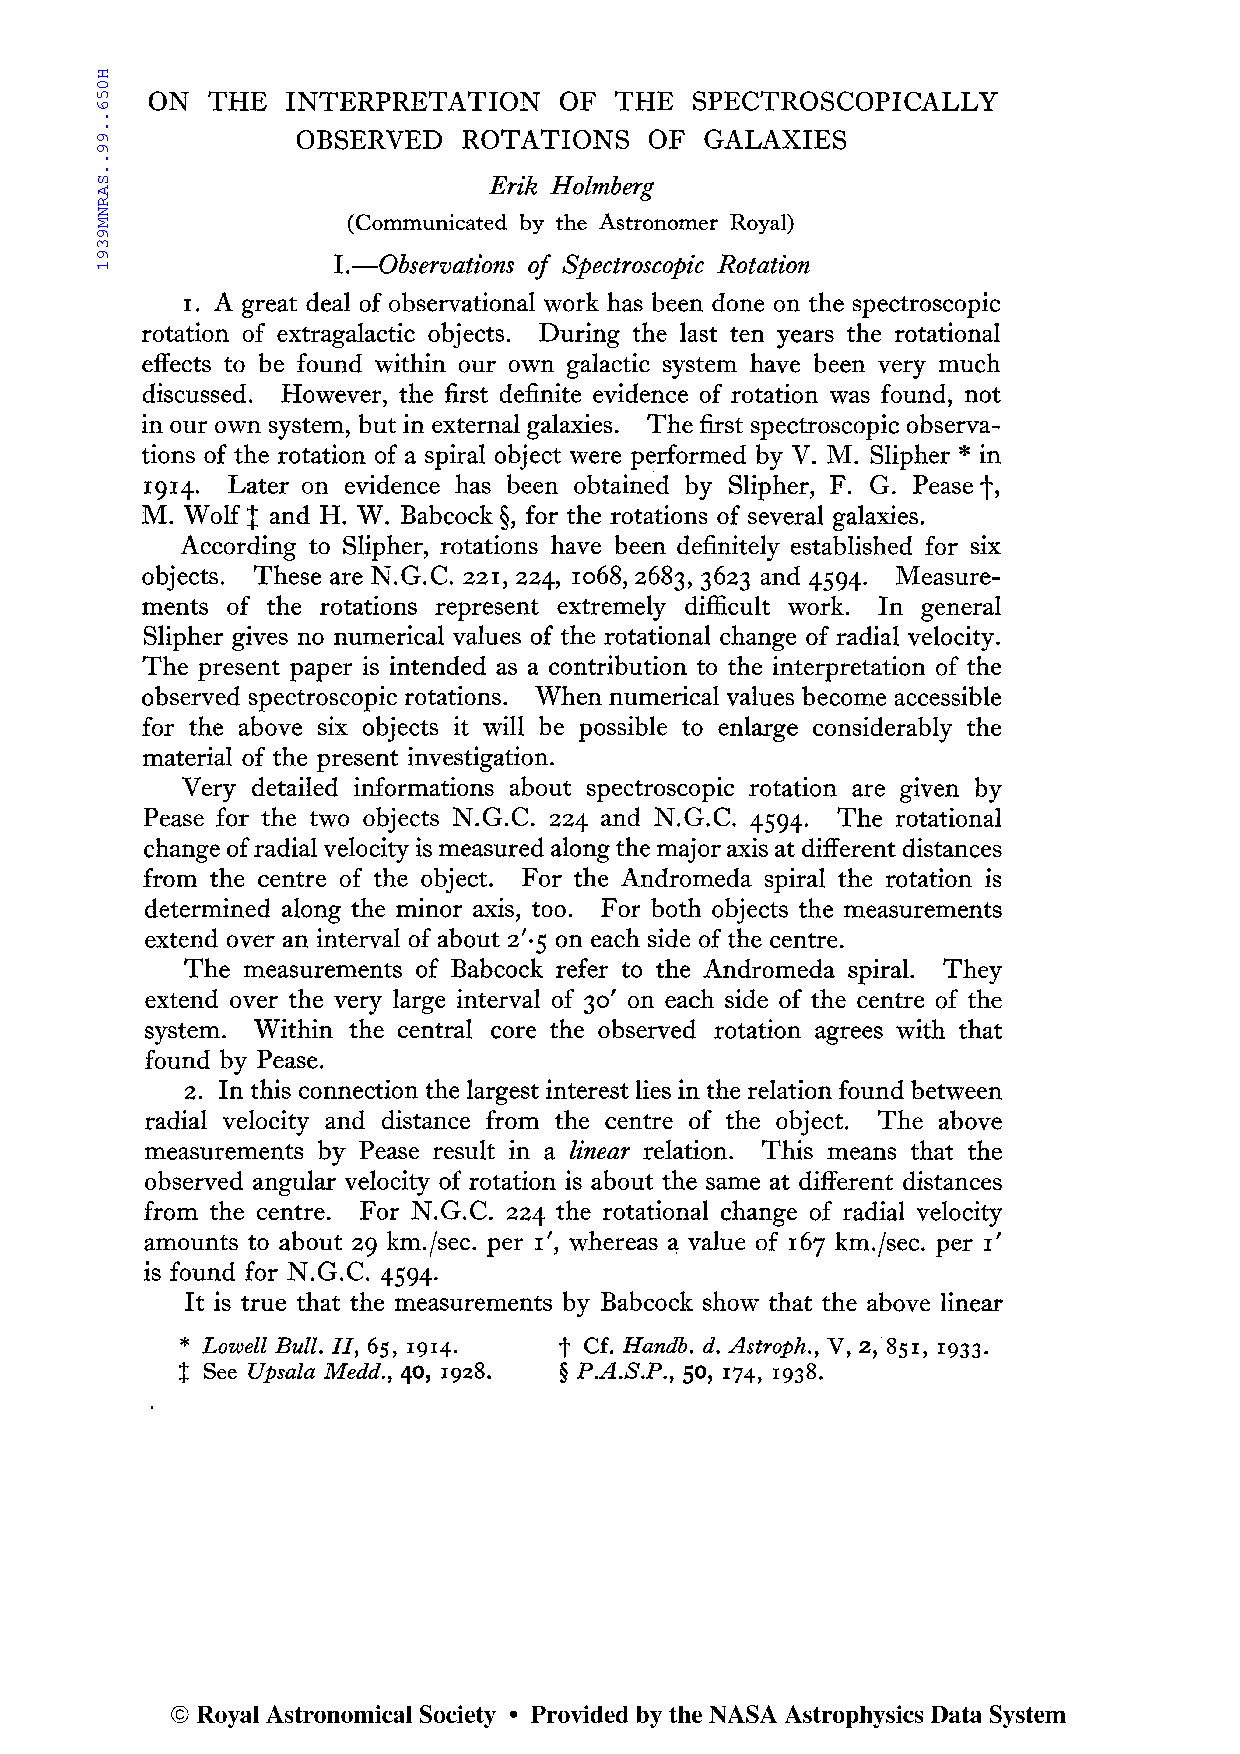
\includepdf[pages=-,width=1.00\textwidth,pagecommand={\thispagestyle{headings}}]{paperI.pdf}
% One additional option could be useful: To cut away the margins of the included PDFs use:
% clip,viewport=<left> <bottom> <right> <top>
% To determine the four numbers you can use the ./determineViewport.sh script in the thesis directory. 

\cleardoublepage
\addcontentsline{toc}{section}{Paper~\II: {\PaperItitle}}

\thispagestyle{empty}

\begin{tikzpicture}[remember picture, overlay]
  \node[fill=black, text=white, font=\bfseries\fontsize{50}{70}, anchor=east, minimum height=1.5cm, minimum width=2cm] at ($(current page.north east) + (0,-0.3\paperheight)$) {\II}; \end{tikzpicture}

\cleardoublepage
% Include the PDF. Comment this while writing the thesis, only add later. 
% Options are: all pages, scaled to full width (use 0.95 if that is too high for some reason), with thesis page number
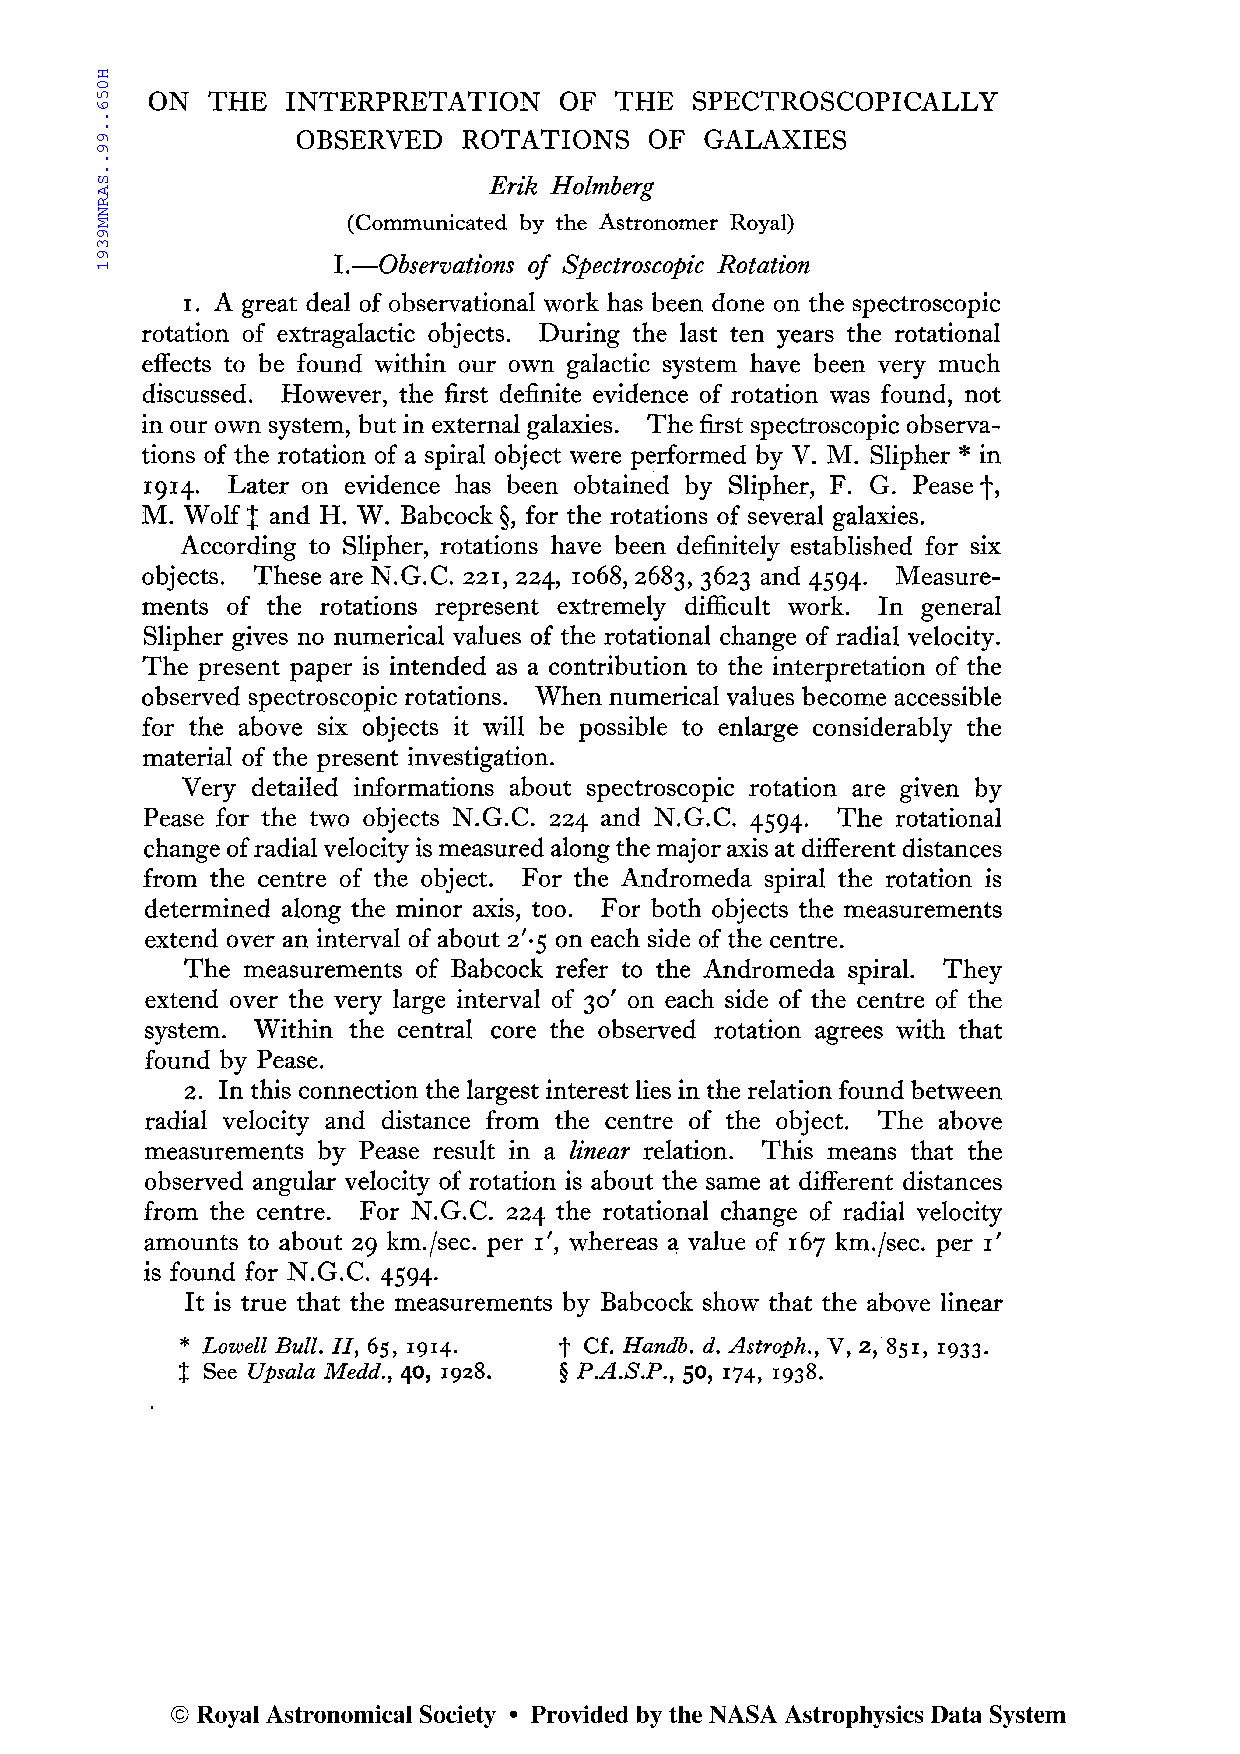
\includepdf[pages=-,width=1.00\textwidth,pagecommand={\thispagestyle{headings}}]{paperI.pdf}
% One additional option could be useful: To cut away the margins of the included PDFs use:
% clip,viewport=<left> <bottom> <right> <top>
% To determine the four numbers you can use the ./determineViewport.sh script in the thesis directory. 

\cleardoublepage

% \appendix
% \thispagestyle{empty}

% \vspace*{4cm} %increase by 2cm each time. %<<<<<<<<<<<<<<<<<<<<<<<<<<<<< Important
% \hfill{ %\fontspec{Frutiger}
%   \fontsize{20}{30}\selectfont {\bf Appendix}}\marginpar{\rule[-4mm]{50mm}{14mm}}
% \vfill

% \begin{tikzpicture}[remember picture, overlay]
%   \node[fill=black, text=white, font=\bfseries\HUGE, anchor=east, minimum height=1.5cm, minimum width=5cm] at ($(current page.north east) + (0,-0.8\paperheight)$) {Appendix};
% \end{tikzpicture}

% \appendix
% \chap{Appendix: Conference posters}
% \section*{Poster 1: \PaperItitle}
% Media-Tryck's suggestion to a poster layout, can be downloaded from \url{https://bildweb.srv.lu.se/login/}.
% Presented 2067 at the \emph{Symposium for time travel}
% in Berlin, Germany. For further details refer to Paper~\I and
% Sect.~\ref{sec:mainresults}.
%
% % include poster itself. Cropping works as described above for the papers.
% 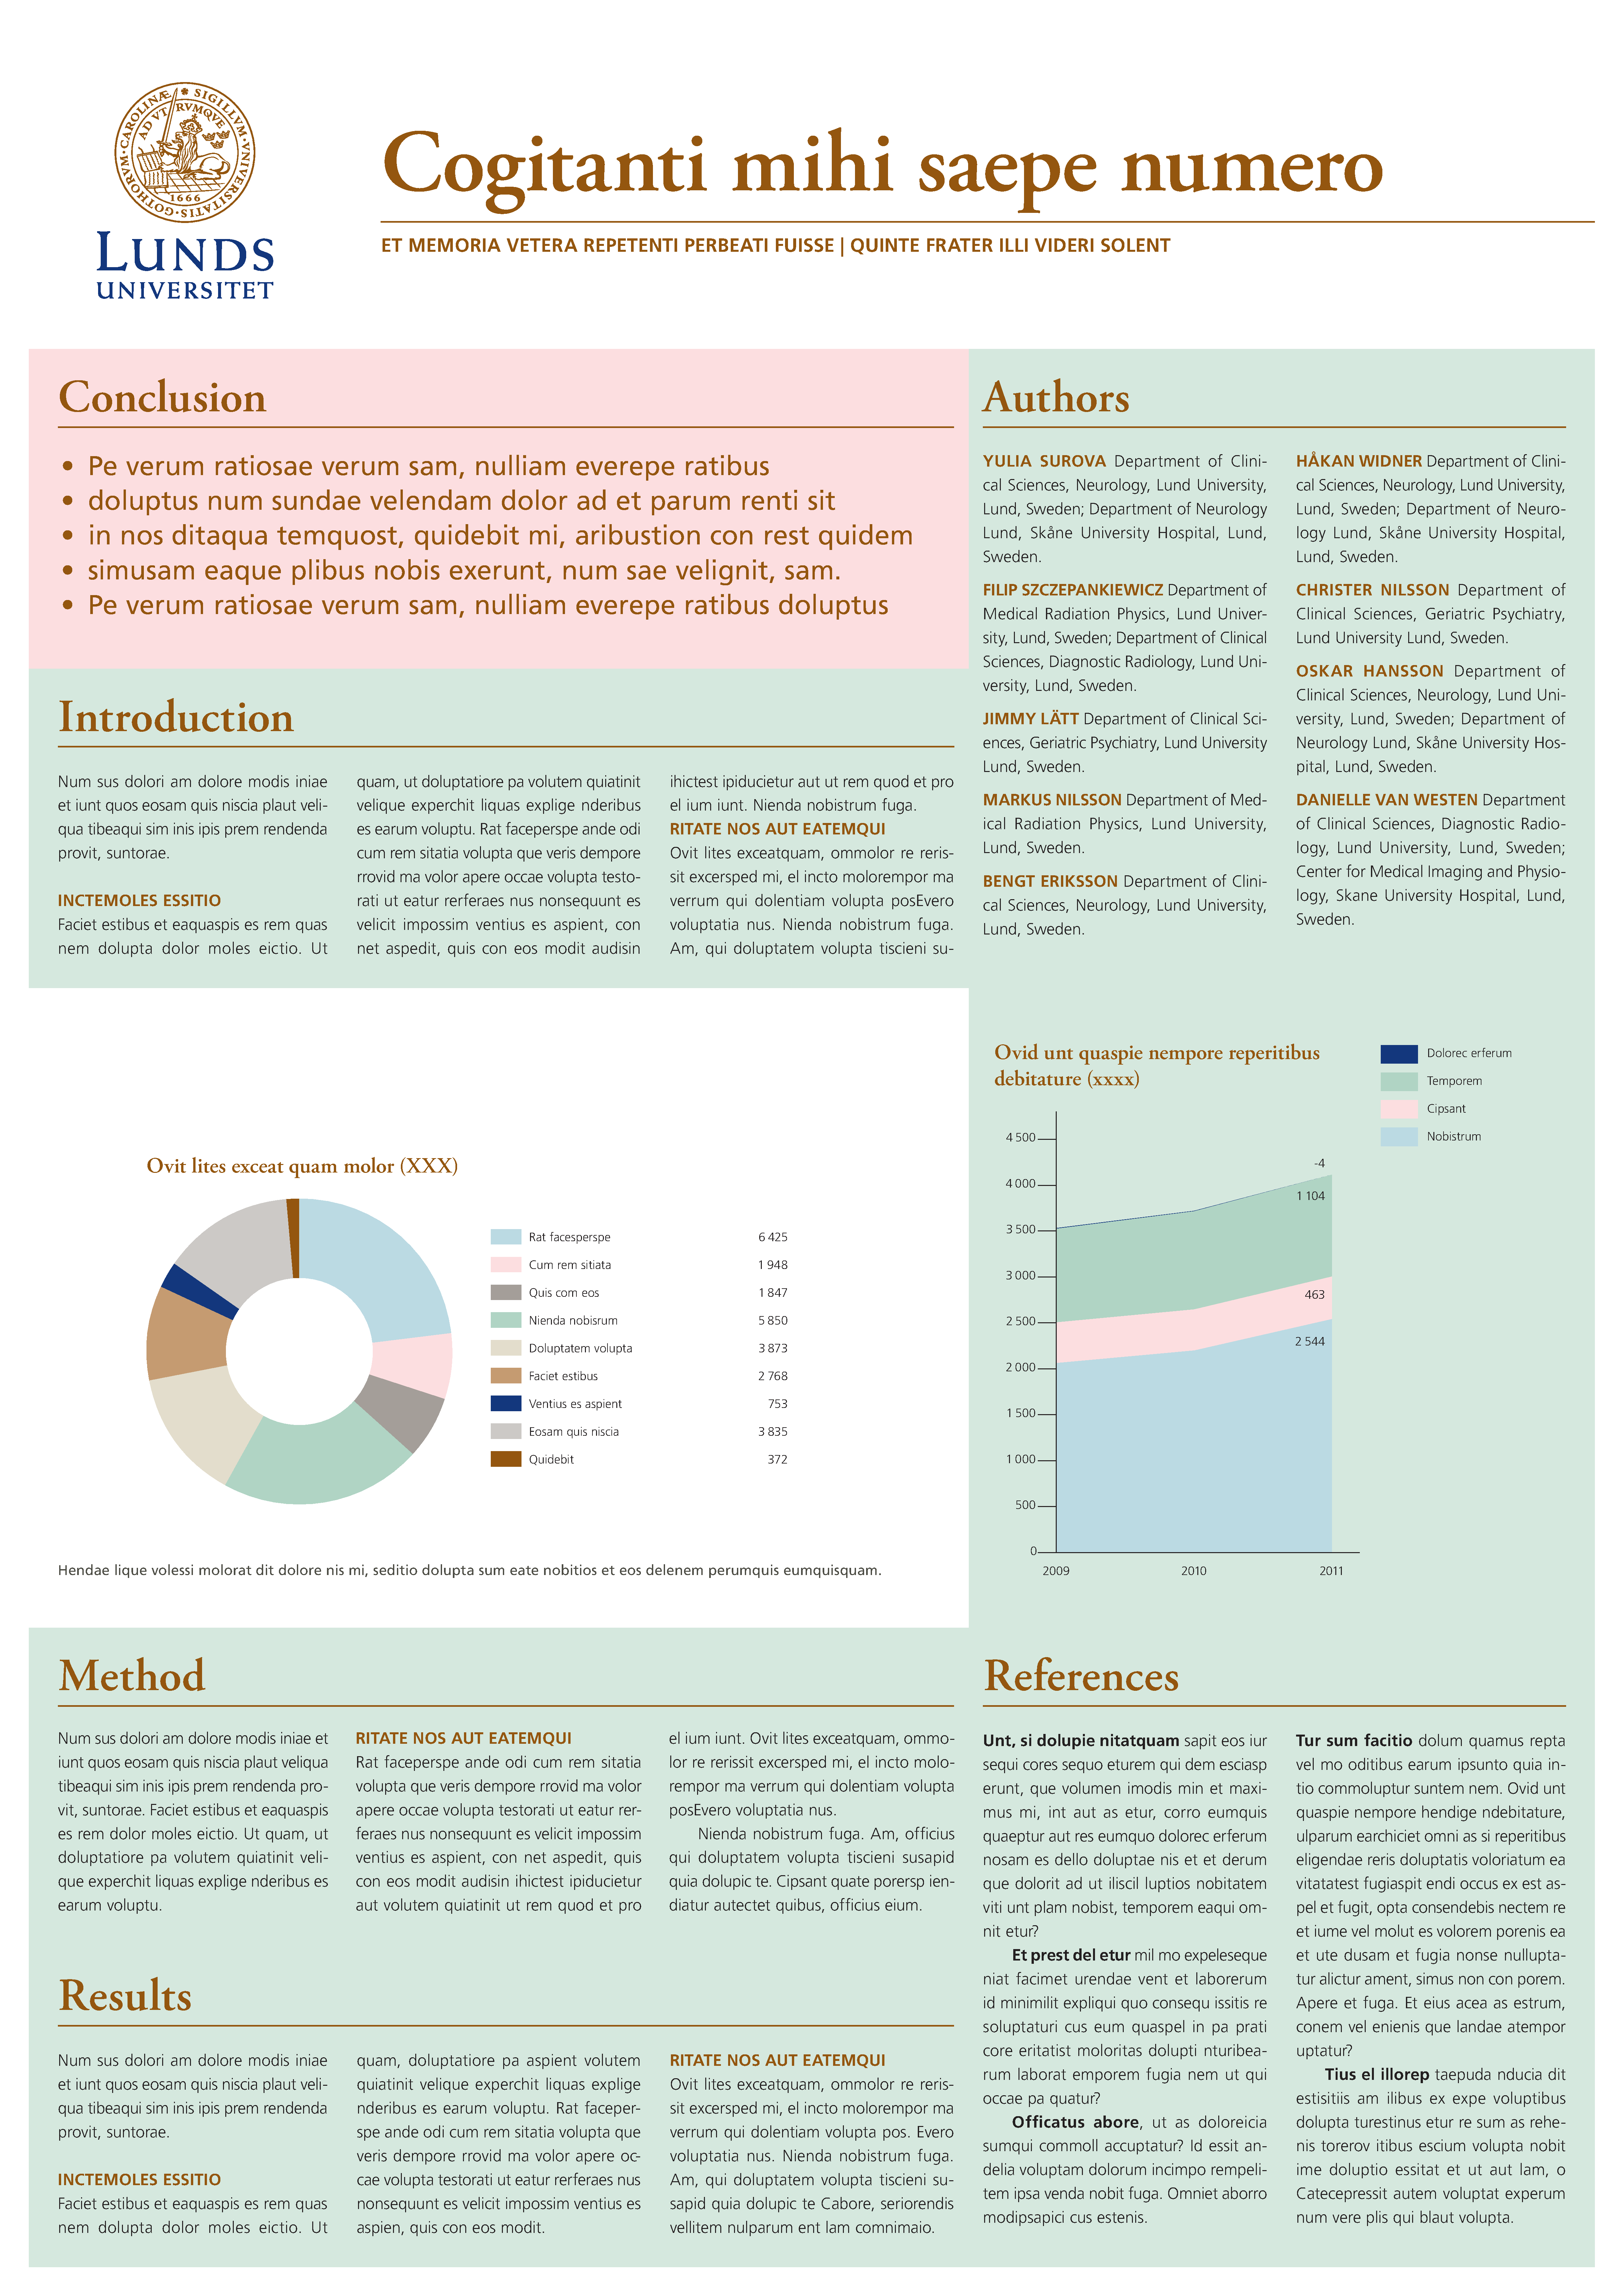
\includepdf[pages=-,width=\paperwidth-10mm]{posterMediaTryck.pdf} %smaller margin, works fine when printing (hopefully ;) Hallå, Jonas!)

\end{document}
